\documentclass[twocolumn,10pt]{asme2ej}

\usepackage{epsfig} 

\title{%
	Personenzentrisches Projektmanagement\\
	\large 
	- \\
	Die Auswirkungen von Projektmanagement in Data Science Projekten\\ 
   auf verschiedene Persönlichkeiten nach dem DISG-Modell}

\author{Tobias Rohrer
    \affiliation{
	Hochschule Darmstadt\\
	Data Science (Master)\\
    Email: sttorohr@stud.h-da.de
    }	
}

\graphicspath{ {./images/} }
\usepackage[center]{caption}
\usepackage[locale=DE]{siunitx}
\usepackage{hyperref}

\usepackage{listings}
\usepackage{xcolor}
\usepackage{enumitem}
\definecolor{codegreen}{rgb}{0,0.6,0}
\definecolor{codegray}{rgb}{0.5,0.5,0.5}
\definecolor{codepurple}{rgb}{0.58,0,0.82}
\definecolor{backcolour}{rgb}{0.95,0.95,0.92}

\lstdefinestyle{mystyle}{
	backgroundcolor=\color{backcolour},   
	commentstyle=\color{codegreen},
	keywordstyle=\color{magenta},
	numberstyle=\tiny\color{codegray},
	stringstyle=\color{codepurple},
	basicstyle=\ttfamily\footnotesize,
	breakatwhitespace=false,         
	breaklines=true,                 
	captionpos=b,                    
	keepspaces=true,                 
	numbers=left,                    
	numbersep=5pt,                  
	showspaces=false,                
	showstringspaces=false,
	showtabs=false,                  
	tabsize=2
}
\lstset{style=mystyle}
\begin{document}

\maketitle    

%%%%%%%%%%%%%%%%%%%%%%%%%%%%%%%%%%%%%%%%%%%%%%%%%%%%%%%%%%%%%%%%%%%%%%
\begin{abstract}


\end{abstract}

%%%%%%%%%%%%%%%%%%%%%%%%%%%%%%%%%%%%%%%%%%%%%%%%%%%%%%%%%%%%%%%%%%%%%%
\section{Einleitung}
Methoden und Werkzeuge zum Managen von Projekten werden meist anhand des Projektumfangs, Komplexität oder der Klarheit von Anforderungen ausgewählt. Außer acht gelassen wird dabei jedoch, dass sich ein Projektteam aus verschiedenen Persönlichkeiten mit unterschiedlichen Stärken und Schwächen zusammen setzt. Einer der Punkte im Agilen Manifesto lautet sogar "Individuals and interactions over processes and tools" \cite{beck2001agile}. Im vorliegenden Bericht wird diskutiert, wie sich verschiedene Projektmanagement-Werkzeuge und Methoden auf die Stärken, Schwächen und die Motivation der Persönlichkeiten nach dem DISC-Modell auswirken. Dazu wird in Abschnitt \ref{sec:1} zunächst kurz auf das Projektmanagement in Data Science Projekten eingegangen und drei geläufige Methoden gegenüber gestellt. In Abschnitt \ref{sec:2} werden anschließend die Persönlichkeitskategorien nach dem DISC-Modell beschrieben. Außerdem wird diskutiert, wie sich die Projektmanagement-Methoden und Werkzeuge aus Abschnitt \ref{sec:1} auf die Stärken, Schwächen und die Motivation der der am Team teilnehmenden Persönlichkeiten auswirkt. Abgeschlossen wird der Bericht mit einem Fazit in Kapitel \ref{sec:3}.


\section{Projektmanagement in Data Science Projekten}\label{sec:1}
Es gibt unzählige Methoden, um Projekte zu verwalten. Im Folgenden werden 3 der meist verbreitetsten kurz beschrieben\footnote{Ausführlichere Beschreibungen der Methoden in den Quellen.}. Anschließend werden die Besonderheiten von Data Science Projekten erläutert und die drei zuvor beschriebenen Methoden im Bezug auf diese Besonderheiten kurz gegenüber gestellt.

\subsection{Wasserfallmodell}
Das Wasserfallmodell lässt sich am besten durch seine sequenziell ablaufenden Phasen charakterisieren. Eine neue Phase wird erst nach erfolgreichem Abschluss der vorgeschalteten Phase gestartet. Zwar bietet das Wasserfallmodell eine gute Übersicht über die Gesamtplanung des Projekts, doch ist es relativ unflexibel gegenüber Veränderungen \cite{Wasserfall}.

\subsection{Agile}
Die Grundideen, sowie Prinzipien des Agilen Projektmanagements ist in dem Agile Manifesto  \cite{beck2001agile} festgehalten. Scrum und Kanban gehören beide zur Gruppe der Agilen Methoden und teilen demnach die Agilen Grundprinzipien.

\subparagraph{Scrum}
Die Grundidee von Scrum ist die Einteilung des Projektes in Inkremente. Jedes Inkrement wird innerhalb eines Sprints fertig gestellt und anschließend an die Kunden ausgeliefert. Somit kann kontinuierlich Rückmeldung des Kunden in den Entwicklungsprozess einfließen. In einem Team, das nach Scrum arbeitet gibt es feste Rollen wie den Product Owner, den Scrum Master sowie das Projekt Team. Dem Product Owner obliegt üblicherweise die inhaltliche und dem Scrum Master die organisatorische Verantwortung \cite{scrum}.

\subparagraph{Kanban}
Angefangene Aufgaben schnellst möglich fertig zu stellen ist eines der zentralen Punkte von Kanban. Um sich auf angefangene Aufgaben zu konzentrieren und deren Fertigstellung zu beschleunigen, wird üblicherweise eine Work in Progress (WiP) Grenze definiert. Alle Aufgaben, sowie deren Status werden auf einem gemeinsamen Kanban Board visualisiert. Aktualisierungen werden an den Kunden ausgeliefert, sobald Sie fertig sind. Im Vergleich zu Scrum kann Kanban als eher kontinuierliche Methode angesehen werden, wobei Scrum mit Sprints arbeitet. Außerdem gibt es keine festgelegten Rollen \cite{kanban}.

\subsection{Besonderheiten von Data Science Projekten}
Bei Data Science Projekten ist zu Projektstart oft nicht genau abzuschätzen, ob und in wie fern die festgelegten Ziele mit den verfügbaren Daten erreicht werden können. Dies liegt unter anderem daran, dass die Qualität der zu verarbeitenden Daten fehleingeschätzt wird. Diese wird in der Praxis eher über- statt unterschätzt. Unter Anderem findet deshalb die Auswahl der einzusetzenden Technologien oft erst im laufe des Projektes statt \cite{agile_pm}. Darüber Hinaus können sich die Anforderungen im Laufe des Projektes ändern. Beispielsweise werden durch die Verarbeitung der Daten neue Möglichkeiten vom Entwicklungsteam aber auch von den Kunden überhaupt erst erkannt. 

\subsection{Die Auswahl einer passenden Methode}

\begin{figure}
	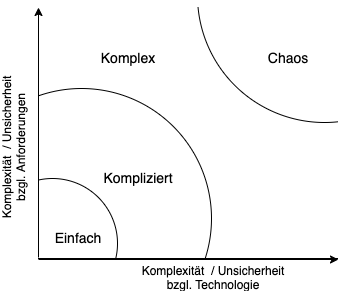
\includegraphics[scale=0.55]{stacey.png}
	\caption[center]{Die Stacey Matrix angelehnt an \cite{stacey_img}}
	\label{fig:stacey}
\end{figure}


Beurteilt man die oben beschriebenen Besonderheiten von Data Science Projekte anhand der Stacey Matrix \cite{Stacey2011StrategicMA}, so finden sich die meisten Projekte mindestens in einem komplizierten, oder eher komplexen Umfeld wieder (siehe Abbildung \ref{fig:stacey}).Um den Unklarheiten in den Anforderungen und der eingesetzten Technologien entgegen zu wirken ist daher der Einsatz einer Agilen Projektmanagement Methode empfehlenswert. Trotzdem hat auch das Wasserfallmodell für Data Science Projekte seinen Anwendungszweck. Beispielsweise könnten starre Unternehmensstrukturen keinen Rahmen für eine Agile Arbeitsweise bieten. Auch könnten Stakeholder eine genaue Planung und Einhaltung des Projektablaufs fordern. 

\section{DISG Projektmanagement}\label{sec:2}
Die Stärken, Schwächen und Motivationsfaktoren der Teammitglieder spielen bei der Wahl einer passenden Projektmanagement Methode üblicherweise keine Rolle. Nach dem  DISG-Modell \cite{disc} setzen sich Persönlichkeiten verschieden stark aus den vier Grundtypen Dominant(D), Initiativ(I), Stetig(S) und Gewissenhaft(G) zusammen. Die verschiedenen Grundtypen nach dem DISG-Modell haben typische Charaktereigenschaften, Stärken, Schwächen, sowie Motivationsfaktoren. Das ein Projektteam besonders effizient ist, wenn die Teilnehmenden motiviert sind und ihre Stärken voll einsetzen können, sollte nicht überraschen. Im Folgenden werden daher die vier Persönlichkeitstypen nach dem DISG-Modell kurz beschrieben und dargelegt, wie sich die Projektmanagement Strategien aus Abschnitt \ref{sec:1} auf die Stärken, Schwächen und die Motivation dieser auswirkt. 

\subsection{Der Dominante}
Der Dominante  wird vor Allem durch Erfolge und Herausforderungen motiviert. Außerdem genießt der Dominante bei der Bewältigung seiner Aufgaben gerne den Freiraum um Risiken einzugehen und um Entscheidungen zu treffen oder zumindest auf diese einzuwirken. Seine größte Stärke ist die zielorientierte Arbeitsweise. Eine seiner Schwächen, die sich jedoch auch positiv auswirken kann, ist die Ungeduld. Außerdem kann seine direkte Art Konflikte im Team auslösen. Es besteht auch die Gefahr, dass der Dominante seine Autorität überschreitet. Zuletzt laufen dominante Persönlichkeiten die Gefahr sich bei der Aufgabenplanung zu überschätzen.

\subsubsection{Im Agilen Umfeld}
Eine neue Software Version an Kunden auszuliefern kann als Teilerfolg eines Teams angesehen werden. Das Prinzip der frühen und kontinuierlichen Auslieferung von Software könnte sich daher motivierend auf den Dominanten auswirken. Seine ungeduldige Eigenschaft kann sich sogar positiv darauf auswirken, diesem Prinzip treu zu bleiben. Ein weiteres Agiles Prinzip, Projekte um motivierte Personen aufzubauen, kann dem Dominanten den nötigen Rahmen geben, um mit seiner zielstrebigen Arbeitsweise das gesamte Team zu bereichern. Durch das Prinzip regelmäßige Reflektionsveranstaltungen durchzuführen, können Konflikten, die durch die direkte Art des Dominanten entstehen, direkt entgegen gewirkt werden.

\subparagraph{Kanban} Das Ziel, angefangene Aufgaben möglichst schnell abzuschließen und dadurch schnell Erfolge zu verbuchen, kann motivierend wirken und der Ungeduld des Dominanten entgegen wirken. Durch die festgesetzte WiP Grenze kann verhindert werden, dass sich der Dominante zu viel auf einmal vornimmt. Es besteht jedoch die Gefahr, dass mangels festgelegter Rollen der Dominante seine Autorität überschreitet, indem er sich über andere Teammitglieder stellt und somit die Zusammenarbeit und Harmonie des gesamten Teams gefährdet. Ach durch das Pull Prinzip besteht die Gefahr, dass sich der Dominante mit Arbeit überlädt.

\subparagraph{Scrum} Sprints können sich motivierend auswirken, da die Erreichung der festgelegten Sprint Ziele als Herausforderung und die Erfüllung als Erfolg angesehen werden kann. Die Visualisierung des Fortschritts durch ein Burndown Chart kann sich hierbei als zusätzlich motivierend auswirken. Der Schwäche, sich zu viel vorzunehmen kann in den Sprint Planing Terminen entgegengewirkt werden. Dabei ist zu beachten, dass die Abschätzung des Aufwands von Aufgaben durch das Entwicklungsteam, wie zum Beispiel mittels Planungspoker, stattfindet. Die durch Scrum fest eingeplanten Retrospektiven können die Wogen, die eventuell durch seine direkte Kommunikation entstehen, direkt geglättet werden. Ist der Hang, seine Autoritäten zu überschreiten stark ausgeprägt, könnte der Scrum Master entgegenwirken.

\subsubsection{Im Wasserfallmodell}
Durch die präzise sequenzielle Planung des Projektes sowie einer festen Projektstruktur, wird zwar der Gefahr entgegengewirkt, dass der Dominante seine Autorität überschreitet und somit Konflikte im Team entstehen. Doch wird durch diese präzise sequenzielle Planung auch die Software erst relativ spät im Entwicklungsprozess an den Kunden ausgeliefert. Dies könnte sich wegen der ungeduldigen Eigenschaft, sowie den fehlenden Teilerfolgen demotivierend auswirken. Des Weiteren würde die sequenzielle starre Planung weniger Freiraum für Risikobehaftete Ideen bringen. Dazu besteht die Gefahr, dass sich der Dominante bei der Anfangsplanung überschätzt und es dadurch zu Fehleinschätzungen im Projektplan kommt.

\subsubsection{Folgerung}
Im Agilen Umfeld fühlen sich Personen mit einer stark ausgeprägten dominanten Eigenschaft unter Anderem wegen der Inkrementellen Arbeitsweise und der damit verbundenen Erfolgserlebnisse wohl. Bei einer Organisation nach Scrum könnte bei einer starken Ausprägung der autoritären Eigenschaft besser als durch Kanban entgegen gewirkt werden. Der Dominante würde sich im Wasserfallmodell, wenn er keine Leitende oder Planende Funktion inne hat eher unwohl fühlen.

\subsection{Die Initiative}
Die Initiative ist in einer Umgebung, in der sie Sichtbarkeit und Popularität im Team aber auch darüber hinaus erfährt, motiviert. Gerne hat sie Raum, um ihre Ideen einzubringen. Wenn sie dabei für ihre Ideen positives Feedback, Anerkennung oder Unterstützung Anderer erfährt, wirkt sich das besonders motivierend aus. Zu den Stärken der Initiativen gehört Kreativität und Impulsivität, was sie zu einer guten Ideengeberin macht. Außerdem kann sie mit ihrer Überzeugungskraft und Optimismus motivierend auf das ganze Team wirken, wodurch sie oft an Popularität in der Gruppe gewinnt. Diese kann sie nutzen um als Schlichterin in der Gruppe zu fungieren. Ist der Hang zur Impulsivität jedoch stark ausgeprägt, können aber auch gerne Details bei der Planung oder Durchführung von Aufgaben übersehen werden. Außerdem kann die Motivation für bereits angefangene Aufgaben verloren gehen, woran die Qualität leiden kann.

\subsubsection{Im Agilen Umfeld}
Das Projekt um motivierte Personen aufzubauen und diese zu unterstützen ist eines der Agilen Prinzipien. Dadurch wird der Initiativen der Raum gegeben, um mit ihren Ideen Andere zu überzeugen und positives Feedback zu ernten. Durch eine üblicherweise enge Zusammenarbeit zwischen Managern und Entwickler während des Projektverlaufs, hat die Initiative die Möglichkeit ihre Sichtbarkeit und Popularität über die Grenzen des Entwicklungsteams hinweg auszubauen. Des weiteren können ihre kreativen Ideen auch noch im laufe des Projektes berücksichtigt werden.

\subparagraph{Kanban} Durch den kontinuierlichen und flexiblen Ablauf bietet Kanban den nötigen Freiraum, um der Initiativen jederzeit die Möglichkeiten zu geben, ihre kreativen Ideen einzubringen. Dabei besteht Gleichzeitig die Gefahr, dass durch die impulsive und überzeugende Art übermäßig viele Umplanungen vorgenommen werden, worunter die Effizienz der Entwicklung leiden kann. Die Visualisierung des aktuellen Entwicklungsstandes auf dem gemeinsamen Kanban Board kann der Initiativen helfen, sich auf die aktuellen Arbeiten zu fokussieren. 

\subparagraph{Scrum} Durch die fest eingeplanten Scrum Events bekommt die Initiative regelmäßig den Raum, um ihre Popularität und Sichtbarkeit in der Gruppe auszubauen. Sprints könnten der Initiativen bei einer starken Ausprägung ihrer impulsiven Eigenschaft den Rahmen geben, sich auf angefangene und festgelegte Aufgaben zu konzentrieren. Jedoch könnte die starre Sprintplanung der Initiativen ein Stück weit den Raum nehmen, um jederzeit ihre kreativen Ideen einzubringen. Durch die Impulsivität und sinkende Motivation für die Fertigstellung von Aufgaben bekommt eine klare Definition of Done eine wichtige Bedeutung um einen Qualitätsmaßstab festzulegen. 

\subsubsection{Im Wasserfallmodell}
Ein klar definierter Projektplan könnte der Initiativen den Rahmen geben um sich besser auf die bevorstehenden Aufgaben zu fokussieren. Jedoch hat sie nicht den Freiraum, um ihre Ideen auch später im Projektverlauf unterzubringen. Durch die klarere Trennung zwischen Entwicklungsteam und Managern hat die Initiative außerdem eine kleinere Audienz, um mit ihren Ideen zu glänzen, was sich motivierend ausüben würde.

\subsection{Folgerung}
Zusammenfassend lässt sich sagen, dass die Initiative sich in einem Agilen Umfeld wohl effizienter einsetzen lässt. Bei Kanban sollte darauf geachtet werden, dass die Initiative durch ihre Impulsivität nicht Chaos auslöst. In Scrum sollte darauf geachtet werden, dass die Initiative auch während eines geplanten Sprints den Raum hat um ihre Ideen einzubringen und Feedback dafür zu bekommen. Das Wasserfallmodell würde sich vor Allem wegen dem fest definierten Projektplan demotivierend auswirken. 


\subsection{Der Stetige}
Der Stetige wird unter Anderem durch die unterstützende Teilnahme an Aufgaben motiviert, ohne dabei aber zwingend als treibende Kraft mitzuwirken. Teammitgliedern zu helfen und dadurch Beziehungen aufzubauen bringt hierbei die Motivation. Eine Anerkennung dieser unterstützenden Art durch das Team wirkt sich hierbei besonders motivierend aus. Zu den Stärken gehört, dass sich der Stetige durch seine empathischen und freundlichen Eigenschaften, sowie der Fähigkeit sich unterzuordnen bestens dafür eignet, um die Kommunikation mit Stakeholdern zu übernehmen. Außerdem nimmt er sich gerne Zeit zuzuhören und nimmt sich auch Probleme anderer an, was ihn zu einem guten Team Player macht. Zu den Schwächen gehört eine gewisse Inflexibilität gegenüber Veränderungen. Des Weiteren besteht die Gefahr, dass sich der Stetige mit Aufgaben überlädt, in der Angst mit einem "Nein" die Harmonie des Teams zu gefährden. Zuletzt kritisiert der Stetige nicht gerne und wird auch nicht gerne kritisiert.

\subsubsection{Im Agilen}
In Agilen Projekten werden Personen und zwischenmenschliche Interaktionen über Prozesse und Tools angeordnet. Diese Priorisierung kann sich positiv auf die Harmonie im Team und somit motivierend. Das Agile Prinzip der technischen Exzellenz, wird unter Anderem durch Code Reviews sicher gestellt. Hierfür bietet sich der Stetige bestens als geduldiger Überprüfer an. Es sollte aber darauf geachtet werden, dass der Stetige berechtigte Kritik anbringt und diese nicht aus Angst die Harmonie zu gefährden zurück hält. Bei dem agilen Konzept, auf Veränderungen zu reagieren, anstatt einem Plan zu Folgen, könnte sich der Stetige jedoch bei zu spontanen Änderungen überrumpelt fühlen.

\subparagraph{Kanban} Angefangene Aufgaben möglichst schnell abzuschließen ist einer der Kernkonzepte von Kanban. Hierbei kann der Stetige durch seine unterstützende Art Anderen helfen, um Tasks abzuschließen. Die daraus entstehenden Beziehungen und Anerkennung würde sich motivierend auswirken. Außerdem wird durch das gemeinsame arbeiten an Aufgaben das Wissen in einem Team verteilt, wodurch weniger Flaschenhälse entstehen und auch zukünftige Tasks schneller abgearbeitet werden können \cite{kanban}. Durch die Fokussierung auf die aktuellen Aufgaben und weniger auf die Planung könnte dem Stetigen jedoch die notwendige Planungssicherheit fehlen.

\subparagraph{Scrum} Die Definition fester Rollen, sowie Sprints könnte dem Stetigen die notwendige Planungssicherheit und Struktur geben, um sich im Agilen Umfeld wohl zu fühlen. In den Regelmäßigen Scrum Events hätte der Stetige den Raum um Beziehungen aufzubauen.

\subsubsection{Wasserfallmodell}
Die Planungssicherheit würde dem Stetigen die Sicherheit geben, um sich wohl zu fühlen. 

\subsubsection{Folgerung}
Im Gegensatz zum Dominanten und zur Initiativen würde sich der Stetige auch im Wasserfallmodell wohl fühlen. Im Agilen sollte darauf geachtet werden, dass Änderungen am Prozess und an der Arbeitsweise transparent und kontinuierlich erfolgt. Scrum könnte durch die Sprints und festen Rollen mehr Sicherheit als Kanban geben. 
 
\subsection{Die Gewissenhafte}
Die Gewissenhafte lässt sich vor Allem durch einen hohen Qualitätsstandard bei der Durchführung von Aufgaben motivieren. Zu den größten Stärken der Gewissenhaften gehört die Gründlichkeit und Ausdauer bei der Bearbeitung von Aufgaben. Auch bei den Aufgaben Anderer testet die Gewissenhafte gerne und bringt Verbesserungsvorschläge ein. Ist ihr Qualitätsbewusstsein jedoch zu stark ausgeprägt kann dies auch ein Nachteil sein. Dann "verkünstelt" sich die Gewissenhafte gerne.

\subsubsection{Im Agilen}
Das agile Prinzip, nachdem durchgängig auf technische Exzellenz und gutes Design geachtet werden soll kommt der Gewissenhaften entgegen. Frühes und kontinuierliches Feedback des Kunden ist zentral im Agilen Umfeld und wird durch eine frühe und kontinuierliche Auslieferung von Software ermöglicht. Durch diese kann es jedoch passieren, dass auch Aktualisierungen an die Kunden ausgeliefert werden, die noch nicht vollkommen perfekt und vollständig sind.  Diese Tatsache könnte sich frustrierend und demotivierend auf die Gewissenhafte auswirken.

\subparagraph{Kanban}
Das Konzept, dass angefangene Aufgaben möglichst schnell abgeschlossen werden sollen könnte dem perfektionistischen Hang der Gewissenhaften entgegen wirken, aber auch demotivierend auf sie wirken.

\subparagraph{Scrum}
Scrum gibt dem Gewissenhaften durch die Sprints in den Rahmen sich für eine bestimmte Zeit auf seine Aufgaben zu fokusieren. Des weiteren würde ein festes Sprintende ein Enddatum für eine Aufgabe darstellen. Die festgelegten Scrum Events könnten aber in den Augen des Gewissenhaften als zu viel soziale Interaktion demotivierend wirken.

\subsection{Im Wasserfallmodell}
Nach deinem festen Plan zu arbeiten würde während der Implementierung zu weniger Abstimmung und sozialer Interaktion führen, was dem Gewissenhaften den Freiraum gibt, sich auf seine Aufgaben zu konzentrieren. Da die Planung im Wasserfallmodell jedoch am Projektanfang stattfindet, werden oft unvorhersehbare Einzelheiten übersehen und es kommt zu Verzögerungen. Dadurch kann es passieren, dass der Gewissenhafte bei der Bearbeitung seiner Aufgaben unter Zeitdruck gerät und deshalb nicht die Aufgaben nicht seinem Qualitätsstandard entsprechend fertigstellen kann.

\subsection{Folgerung}
Im Agilen Umfeld sollte dem Gewissenhaften der Wert der frühen und kontinuierlichen Auslieferung von Aktualisierungen und des dadurch entstehenden Feedbacks klar gemacht werden. Das Wasserfallmodell würde ihm zwar den Freiraum geben, führt aber bei einer ungenauen Planung zu Zeitdruck, unter dem der Gewissenhafte seinem Qualitätsstandard nicht gerecht werden kann.

\cite{disc_pm}
\section{Fazit}\label{sec:3}

Wie oben dargelegt, fühlen passen verschiedene DISG-Grundtypen zu unterschiedlichen Projektmanagement-Methoden und Werkzeugen. Es ist daher empfehlenswert sich vor der Projektplanung Gedanken darüber zu machen, um die Teammitglieder möglichst effizient einsetzen zu können. Außerdem können durch solche Überlegungen Konflikte im Team vorgebeugt werden. 

In der Praxis kommt selten eine reine Form der drei beschriebenen Methodiken zum Projektmanagement zum Einsatz. Auch bei Mischformen  können die Motivationsfaktoren, Stärken und Schwächen der beteiligen wie oben dargelegt berücksichtigt werden, um ein effizientes Team aufzubauen.

Klar sollte sein, dass in echten Personen immer mehrere Persönlichkeitstypen vorhanden und auch unterschiedlich stark ausgeprägt sind. Trotzdem kann eine Analyse der Persönlichkeiten und die Berücksichtung der Motivationsfaktoren, Stärken und Schwächen dazu beitragen, ein funktionierendes Team aufzubauen.

\bibliographystyle{asmems4}

% Here's where you specify the bibliography database file.
% The full file name of the bibliography database for this
% article is asme2e.bib. The name for your database is up
% to you.
\bibliography{pm}

\end{document}
